\documentclass{article}
\usepackage{multicol}
\usepackage[utf8]{inputenc}
\usepackage{float}
\usepackage{graphicx}
\usepackage{hyperref}
\hypersetup{
    colorlinks=true,
    urlcolor=blue,
    linkcolor=blue,
}

\usepackage{geometry}
\geometry{
    a4paper,
    total={170mm,257mm}
}

\usepackage{forest}
\definecolor{folderbg}{RGB}{124,166,198}
\definecolor{folderborder}{RGB}{110,144,169}
\def\Size{4pt}
\tikzset{
    folder/.pic={
        \filldraw[draw=folderborder,top color=folderbg!50,bottom color=folderbg]
        (-1.05*\Size,0.2\Size+5pt) rectangle ++(.75*\Size,-0.2\Size-5pt);
        \filldraw[draw=folderborder,top color=folderbg!50,bottom color=folderbg]
        (-1.15*\Size,-\Size) rectangle (1.15*\Size,\Size);
    }
}

% ------------------------------- FRONT MATTER ------------------------------- %

\title{\textbf{GreenBook}\\~\\
Third assignment\\
\small Software Development Process course\\
University of Milano - Bicocca\\
A.A. 2021/22\\~\\
\href{https://gitlab.com/massimino96/2021_assignment3_greenbook/}{Repository Link}}
\author{Authors:\\
830260 - Binda Paolo - \href{mailto:p.binda@campus.unimib.it}{p.binda@campus.unimib.it}\\
831075 - D'Apa Massimo - \href{mailto:m.dapa@campus.unimib.it}{m.dapa@campus.unimib.it}\\
830065 - Fornaro Alessandro - \href{mailto:a.fornaro1@campus.unimib.it}{a.fornaro1@campus.unimib.it}}
\date{}

% ------------------------------- DOC. START ------------------------------- %

\begin{document}
    \setlength{\parindent}{0em}
    \setlength{\parskip}{1em}

    \maketitle
    \thispagestyle{empty}

    \cleardoublepage
    \setcounter{page}{1}

    \section*{Introduction}

    Due to the outbreak of the recent COVID-19 pandemic, restaurant owners have found
    themselves facing many new challenges for guaranteeing safety in the workplace for both
    customers and employees alike. And while many of these situations require a practical
    solution, like making sure there's enough distance between tables and that everybody
    is wearing a mask or authenticating green pass certificates at the entrance, others, like
    storing contact trace information, require a more careful approach and a long-term
    strategy is best suited to handle them.


    We developed a web-app, called \textit{GreenBook}, to meet the needs of restaurant
    managers throughout this pandemic. By storing the contact trace information of every
    customer and recording the employees present in the restaurant on a particular
    date and shift we are able to guarantee, in the event of a Covid-19 positive case,
    perfect traceability of all the people that need to be contacted.


    The following ER-schema explicits the entities and relations that we intended
    to model with our application.

    \vspace{5mm}
    \begin{figure}[H]
        \centering
        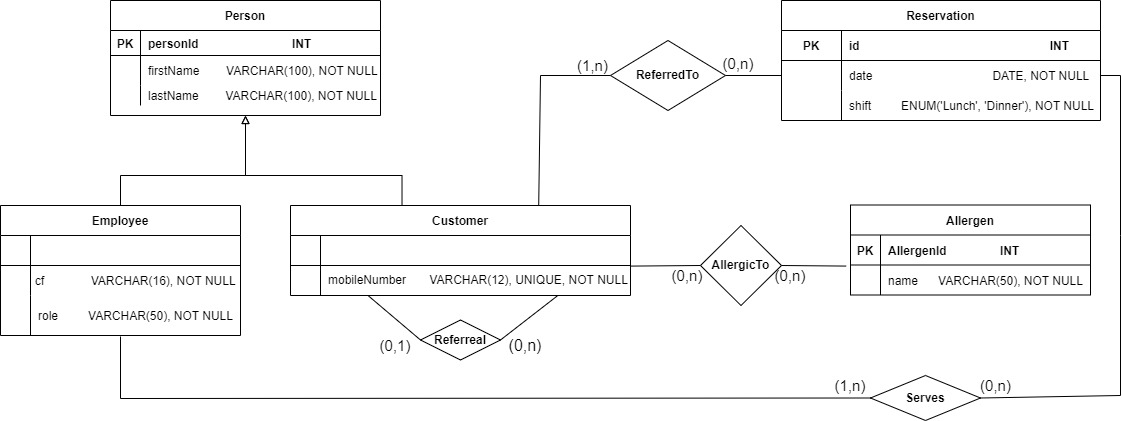
\includegraphics[width=\textwidth]{images/er_model.jpg}
        \label{fig:ermodel}
        \caption{ER Model}
    \end{figure}


\vspace{5mm}
In the phase of ER Design, we made the following assumptions:
\begin{itemize}
  \item A user cannot recommend himself
  \item Tracing also employees which are selected for each reservation should be useful, since they could be infected and, in such cases, we need to be able to track them too
  \item Each customers' credentials are asked during the booking process, so that every person relating to a reservation gets recorded
  \item A restaurant could find useful to register also customers' allergies, 
  in order to avoid needing another application just for this purpose: we implemented this feature even if it is not the functionality for which it was intended.
  \item In our model we allow multiple customer objects to have the same pair of
  first and last name (because this might very well happen in practice) but consider
  the mobile number as a unique identifier, necessary for contacting them.
\end{itemize}


    \newpage

    \section*{Web-app Functionalities}
    The web-app functionalities are divided into four main areas:
    \begin{itemize}
        \item Manage reservations: it is the core functionality of the web-app. It allows
        to record new bookings, search for booked reservations and eventually
        modify or delete them.
        \item Manage employees: this functionality allows the restaurant staff to manage the actual employees, that is, add, edit or remove an employee.
        \item Manage customers: the staff can also see the list of all the customers registered in the restaurant database, insert new customers, edit them and delete them.
        \item Manage allergens: although it is not a core feature for the application, every customer has his special needs and this web-app permits to record possible allergies of each customer.
    \end{itemize}


    We now go through the functionalities offered by our web-app in more detail.

    \subsection*{Manage customers and employees}
    A comfortable overview is provided to the restaurant manager who intends, for whatever reason, to manage employees and customers. In the two sections of the web app it is possible to consult a list of all employees and customers with the possibility of modifying and deleting the data recorded in the system.

    \begin{figure}[H]
        \centering
        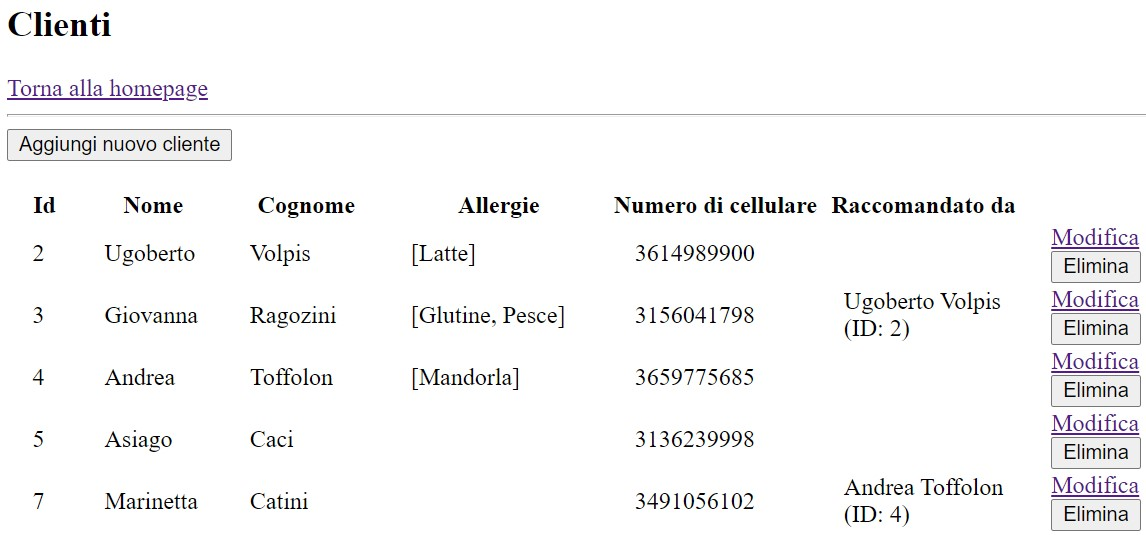
\includegraphics[width=0.8\textwidth]{images/customers_overview.jpg}
        \label{fig:customers_overview}
        \caption{Overview of customers registered in system database}
    \end{figure}

    The two entities are in fact managed in a similar way, allowing the main functions that one would expect to be available to such a staff member:

    \begin{itemize}
        \item Register new employee/customer: in the case of the employee, name, surname, role and fiscal code are required; on the other hand, if it's a customer, it is required to insert name, surname, mobile number and (eventually) the referreal customer, as well as any allergies to watch out for.
        \item Edit employee/customer: it's possible
        to edit a particular person by pressing on the edit button, on the right side of the record, as can be seen in the figure \hyperref[fig:customers_overview]{over here}.
        \item Delete employee/customer: it's possible
        to remove a person from the system by pressing on the remove button, just below the edit button.
    \end{itemize}

    All the values entered by the user are validated by means of specific annotations on the attributes of the classes. Any validation requirement that is violated leads to the appearance of an error and the request to modify the data in the appropriate format, as shown in the figure available at \hyperref[fig:customer_validation_error]{Appendix A: Customer validation error}.


    \subsection*{Manage allergens}
    A comfortable overview is also provided to the restaurant manager for the management of allergens. In the dedicated section of the web app it is possible to consult a list of all of all allergens with the possibility of adding, modifying and deleting new allergens.

\vspace{5mm}

    \begin{figure}[H]
        \centering
        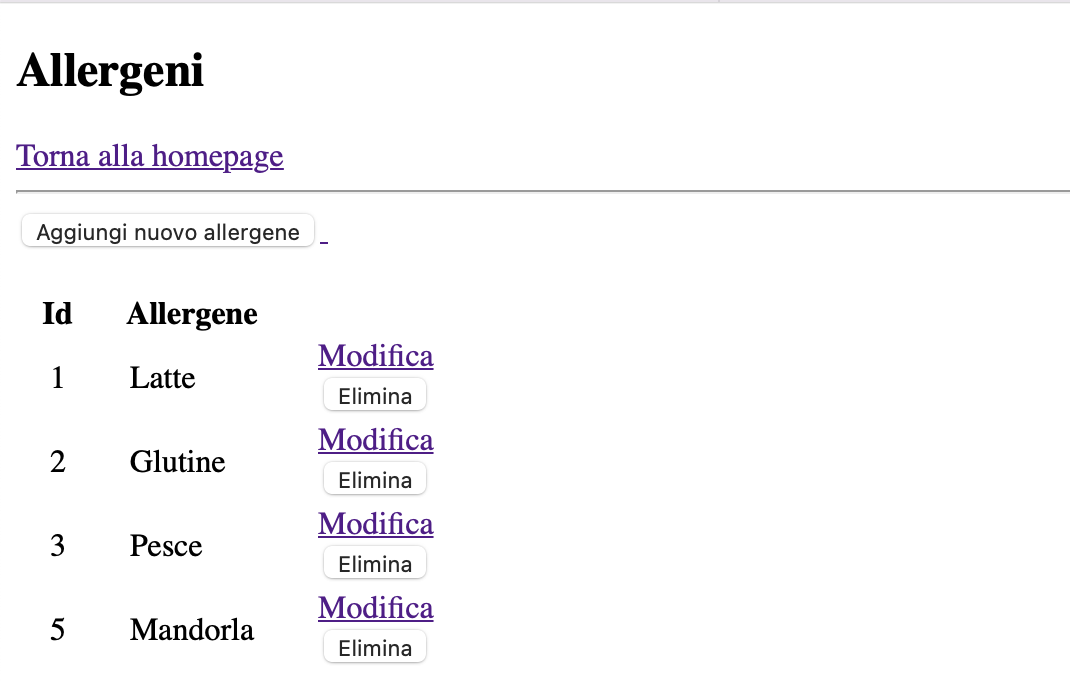
\includegraphics[width=0.8\textwidth]{images/allergens_overview.png}
        \label{fig:allergens_overview}
        \caption{Overview of allergens registered in system database}
    \end{figure}

\vspace{5mm}

    \begin{itemize}

        \item Register new allergen: When registering a new allergen, the name of the allergen is requested. If the allergen being created is already present in the database, an error message will be shown.

        \item Edit allergen: it's possible
        to edit a particular allergen by pressing on the edit button, on the right side of the record, as can be seen in the figure \hyperref[fig:allergens_overview]{over here}. As in the previous case, an error message will be shown if the allergen name being changed is already used, as shown in the figure available at \hyperref[fig:allergen_validation_error]{Appendix A: Allergen validation error}.

        \item Delete allergen: it's possible
        to remove an allergen from the system by pressing on the remove button, just below the edit button, as can be seen in the figure \hyperref[fig:allergens_overview]{over here}. If the allergen is associated with a customer, an error will be shown (\hyperref[fig:allergen_constraint_error]{Appendix A: Allergen constraint error}).

    \end{itemize}

\newpage
    \subsection*{Manage reservations}
    In the manage reservations area of the web-app we can go down three 
    different paths, corresponding to three main functionalities of 
    our application, two lead to searching a reservation in the 
    database, while the other allows the creation of a new one:
    
    \vspace{5mm}
        \begin{figure}[H]
        \centering
        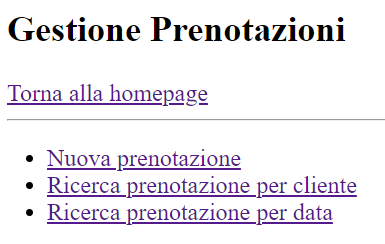
\includegraphics[width=0.5\textwidth]{images/manage_reservations}
        \label{fig:search_reservation_by_customer_errors}
        \caption{Manage reservations}
    \end{figure}
    \vspace{5mm}
    
    
    A more detailed explanation of each functionality is now provided:

    \begin{itemize}
        \item New reservation: allows to create and save a new reservation object.
        During creation we have to select the date and shift of the booking.
        We must add at least one customer (with its mobile
        number) and select at least one employee which will be assigned to serve
        the reservation's customers.
        Failing to meet these requirements will halt the saving
        process and prompt the relative errors
        (\hyperref[sec:new_reservation_form_errors]{Appendix A: New Reservation}.)
        to appear in the form.
        By recording the information this way we are sure, in the case of
        a positive case of Covid, we are able to contact each person that
        was in contact with the infected person.


        \item Search reservation by customer: allows to retrieve all the saved
        reservations in which that customer took part.
        It requires the first and last name of a person.
        Failing to meet these requirements will stop the search process
        and prompt the relative errors
        (\hyperref[sec:search_reservation_by_customer_errors]
        {Appendix A: Search Reservation by Customer})to appear in the form.
        Returns all reservations containing a customer that match
        those credentials (if any).

        \item Search reservation by date: allows to retrieve all the saved reservations
        which took or will take place on a given date.
        It requires a date. Failing to meet this requirement will stop the search
        process and prompt the relative errors
        (\hyperref[sec:search_reservation_by_date_errors]{Appendix A: Search Reservation
        by Date}) to appear in the form.
        Returns all reservations booked for that particular date,
        regardless of the shift (if any).

        \item Edit reservation: in the page where the results of a search are shown,
        all the data relative to a reservation is displayed and it's possible
        to edit (or delete entirely) a particular reservation.
        In the editing process all parts of a reservation can be modified:
        we can add, remove or edit customers, change the reservation's date and shift,
        as well as the employees involved. This process is also subject to the
        above requisites for a saving a reservation.
    \end{itemize}



    \clearpage
    \section*{Source code elements}
    \begin{multicols}{2}
    {\footnotesize\noindent
        \begin{forest}
            for tree={
                font=\ttfamily,
                grow'=0,
                child anchor=west,
                parent anchor=south,
                anchor=west,
                calign=first,
                inner xsep=7pt,
                edge path={
                    \noexpand\path [draw, \forestoption{edge}]
                    (!u.south west) +(7.5pt,0) |- (.child anchor) pic {folder} \forestoption{edge label};
                },
                file/.style={edge path={\noexpand\path [draw, \forestoption{edge}]
                (!u.south west) +(7.5pt,0) |- (.child anchor) \forestoption{edge label};},
                inner xsep=2pt,font=\ttfamily
                },
                before typesetting nodes={
                    if n=1
                        {insert before={[,phantom]}}
                        {}
                },
                fit=band,
                before computing xy={l=15pt},
            }
            [GreenBook
            [src/main/java/it.unimib.bdf.GreenBook
            [controllers
            [AllergenController]
            [CustomerController]
            [EditReservationController]
            [EmployeeController]
            [NewReservationController]
            [ReservationController]
            [SearchReservationController]
            ]
            [models
            [Allergen]
            [Customer]
            [Employee]
            [Person]
            [Reservation]
            ]
            [containers
            [ReservationListContainer]
            [DateContainer]
            ]
            [repositories
            [AllergenRepository]
            [CustomerRepository]
            [EmployeeRepository]
            [ReservationRepository]
            ]
            [services
            [AllergenService]
            [CustomerService]
            [EmployeeService]
            [ReservationService]
            ]
            [GreenBookApplication.java, file]
            [\dots, file]
            ]
            [resources/WEB-INF
            [jsp
            [allergen]
            [customer
            [customers.jsp, file]
            [new-customer.jsp, file]
            [edit-customer.jsp, file]
            ]
            [employee]
            [reservation
            [edit]
            [new]
            [search]
            [reservations.jsp, file]
            ]
            [error.jsp, file]
            ]
            [index.html, file]
            ]
            [\dots, file]
            ]
        \end{forest}
    }\columnbreak

    The code we have developed is mainly divided into two categories: the one necessary for the implementation of the back-end, written in Java, and the one for the front-end, written in JSP (and of course HTML, CSS and JS). The former is located in the \textit{java/src} directory, while the latter is located in \textit{resources/WEB-INF}.

    \subsection*{Front-end}
    The front-end was created by defining a page for each functionality offered by the application. Each of these is in fact dedicated to carrying out CRUD operations on specific entities (allergen/customer/employee). The pages in the reservation directory allow the insertion and search of reservations, thus also implementing operations that require the involvement of multiple database entities.

    \subsection*{Back-end}
    The back-end is dedicated to the management of GET and POST requests made by by the user through the forms presented in the View. There are three foundamental elements associated to each model defined in the code: \textbf{repositories} (persistence logic); \textbf{services} (business logic); \textbf{controllers} (presentation layer).

    \subsubsection*{Repositories}
    In the repositories we placed mechanisms for storage, retrieval, search, update and delete operations. The interfaces defined as repositories are extending \textit{CrudRepository}, which is an interface for generic CRUD operations on a repository for the specific type passed by parameter (eg. Customer).

    Our repository is an in-memory database, made persistent, run by the \textit{H2 Engine}: it provides a Java SQL database and allows to use JDBC to access and manage entities persistence.

    \subsubsection*{Services}
    These classes encapsulate business logic and changes to be persisted to ensure consistent data and the integrity of relationships between entities.
    The purpose of this element is also to define a central point of access to persisted data: all the operations defined in the repository are made available to the controllers through the service.

    \end{multicols}

    \subsubsection*{Controllers}
    The controllers are the managers of the \textit{View}, and provide entry points for GET and POST requests coming from the user. They validate the data provided in the JSP forms and return the appropriate web page, eventually an error page, making sure that data provided by user is consistent with the costraints defined by annotations in the entities.

    \vspace{10mm}
    \section*{Responsibilities of code sections}
    The web app code is broken down into many components and classes, but some of them deserve more attention than others. Therefore, a brief explanation of some parts of the code that have more responsibility than others will be given below.

    \subsection*{Models}
    \textit{Allergen.java, Customer.java, Employee.java} are the implementations of, respectively, the allergen, customer and employee entitites of the ER Model.

    \textit{Person.java} is the parent class of Customer and Employee models, which makes it possible to define only a few additional attributes for these specialized classes. All the attributes of the Person class are in fact inherited and are an integral part of the objects registered in the database: the annotation \textit{@MappedSuperclass}, placed in \textit{Person} class, tells JPA to include the base class properties as if they were declared by the child classes \textit{(Employee, Customer)} extending Person.

    \textit{Reservation.java} is the java class that represents
    the Reservation entity displayed in the above ER, with those attributes and relations
    (annotated with javax persistance commands).

    \subsection*{Controllers}
    Being conprehensive of multiple functionalities and parts, there are four different
    controllers that handle the reservations:

    \begin{itemize}
        \item \textit{ReservationController.java} : handles the page where the possible
        options are displayed and dispatches the requests to the relative jsp accordingly.

        \item \textit{NewReservationController.java} : handles the part related to the
        creation and validation of a new reservation object and saving that
        record to the db.

        \item \textit{SearchReservationController.java} : has the job of searching a
        reservation in the database based on the search parameters (customer or date) and
        showing the search results to the user.

        \item \textit{EditReservationController.java} : controls the process of editing
        a reservation and updating it's record into the db.

    \end{itemize}



    \subsection*{Services}
    \textit{ReservationService.java} dispatches the reservation controllers' query requests to the reservation's repository
    and makes sure that saving a reservation occurs in a transaction.


\subsection*{Repositories}
The \textit{ReservationRepository.java} takes care of actually executing the CRUD queries
asked by the service and implements a few custom queries to meet the application needs.
In particular, here, we hardcoded the sql query that fetches from the database
all the reservations in which a customer, with given first and last name, took part.
This query contains a nested query with a join on two tables and is shown below:

\vspace{5mm}

\begin{figure}[H]
    \centering
    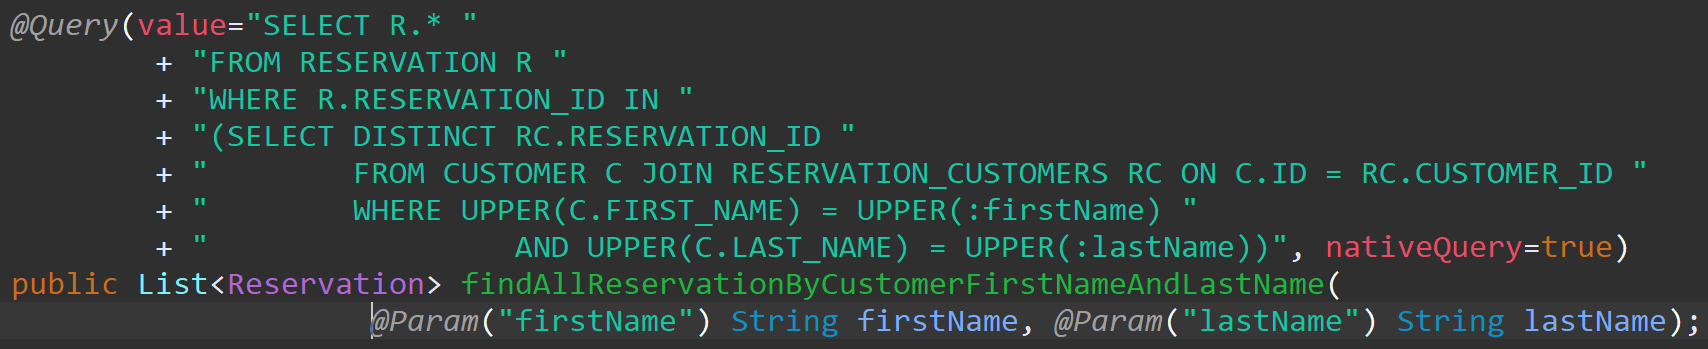
\includegraphics[width=0.9\textwidth]{images/custom_query}
    \label{fig:custom_query}
    \caption{Query for searching the reservations by customer's first and last name.}
\end{figure}








    \newpage
    \section*{Appendix A: Form errors}


    \vspace*{5mm}

    \subsection*{User modification}
    \begin{figure}[H]
        \centering
        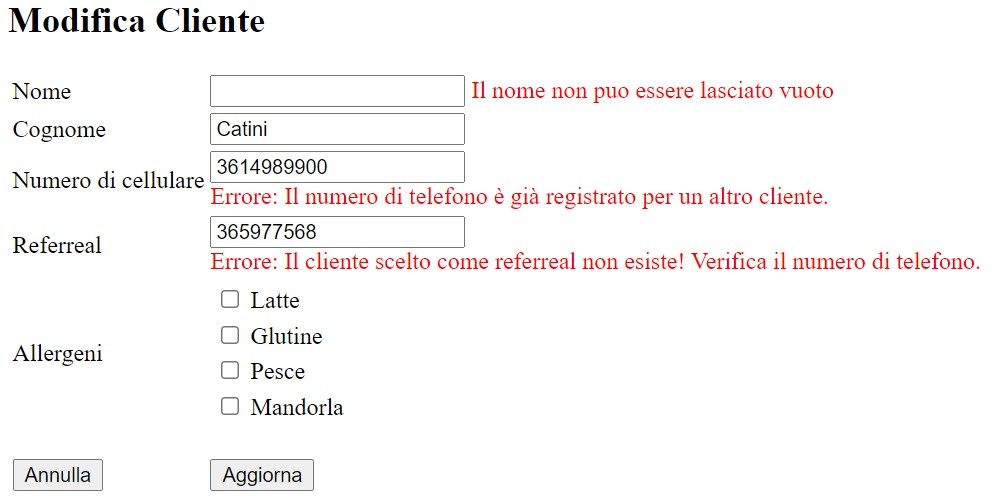
\includegraphics[width=0.9\textwidth]{images/customer_validation_error.jpg}
        \label{fig:customer_validation_error}
        \caption{Customer modification violating requisites}
    \end{figure}

    \vspace*{5mm}

    \subsection*{New Reservation}
    \label{sec:new_reservation_form_errors}
    \begin{figure}[H]
        \centering
        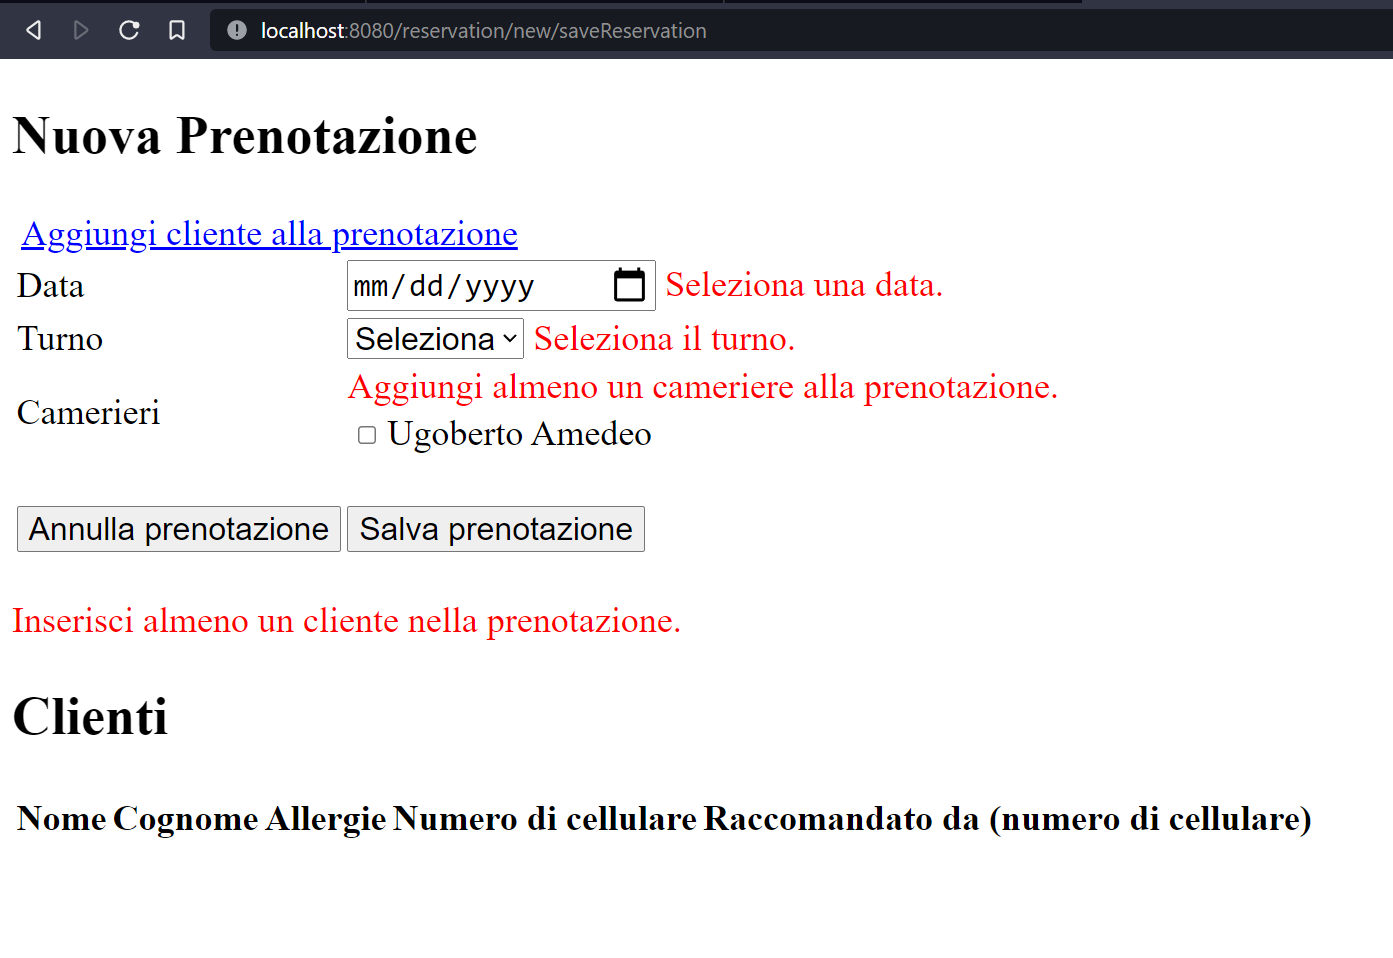
\includegraphics[width=0.9\textwidth]{images/new_reservation_form_errors}
        \label{fig:new_reservation_form_errors}
        \caption{Saving a new reservation violating requisites}
    \end{figure}

    \vspace*{5mm}

    \subsection*{Allergen modification}
    \begin{figure}[H]
        \centering
        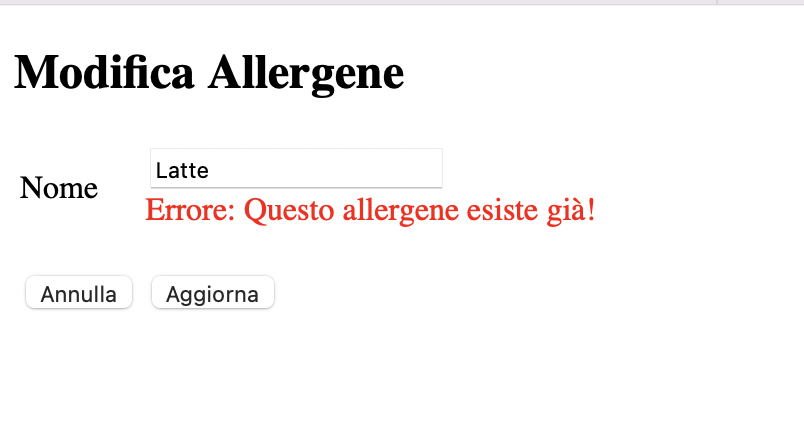
\includegraphics[width=0.9\textwidth]{images/allergen_validation_error.png}
        \label{fig:allergen_validation_error}
        \caption{Allergen modification violating requisites}
    \end{figure}

    \vspace*{5mm}

    \subsection*{Allergen deleting}
    \begin{figure}[H]
        \centering
        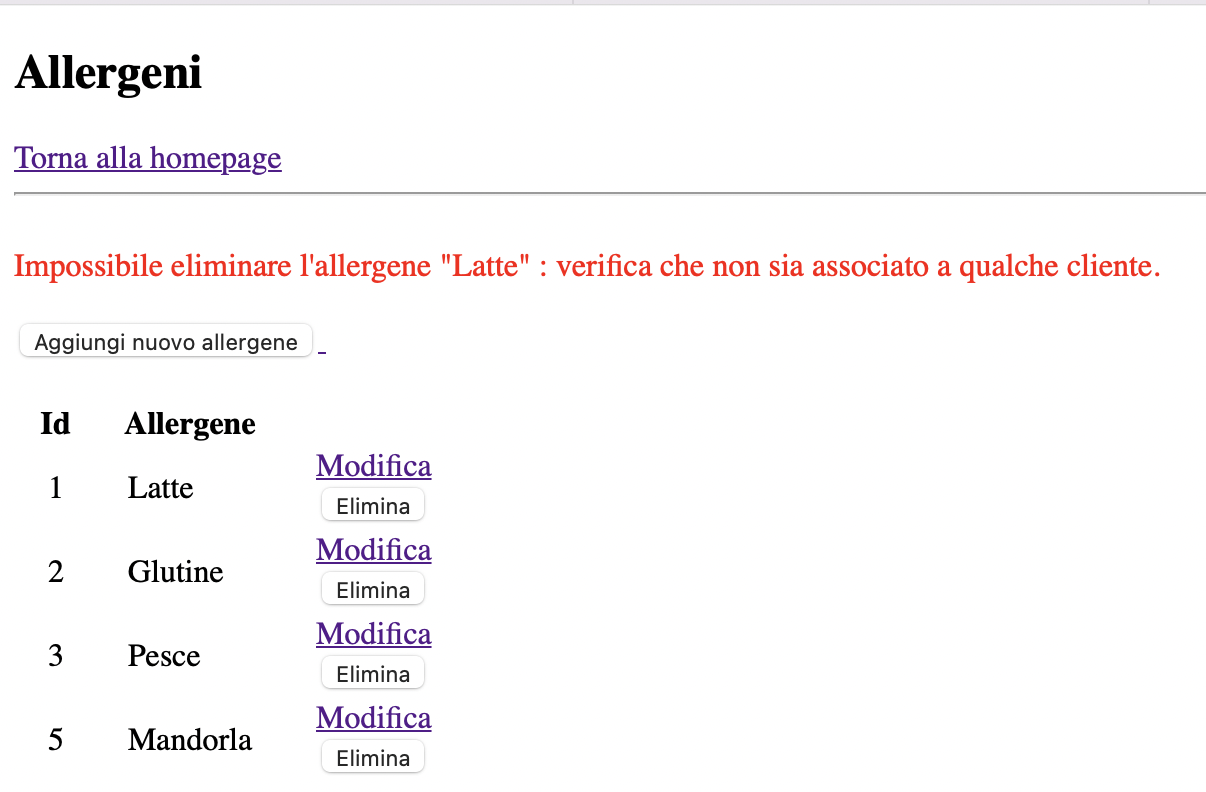
\includegraphics[width=0.9\textwidth]{images/allergen_constraint_error.png}
        \label{fig:allergen_constraint_error}
        \caption{Allergen constraint error}
    \end{figure}


    \subsection*{Search Reservation by Customer}
    \label{sec:search_reservation_by_customer_errors}
    \begin{figure}[H]
        \centering
        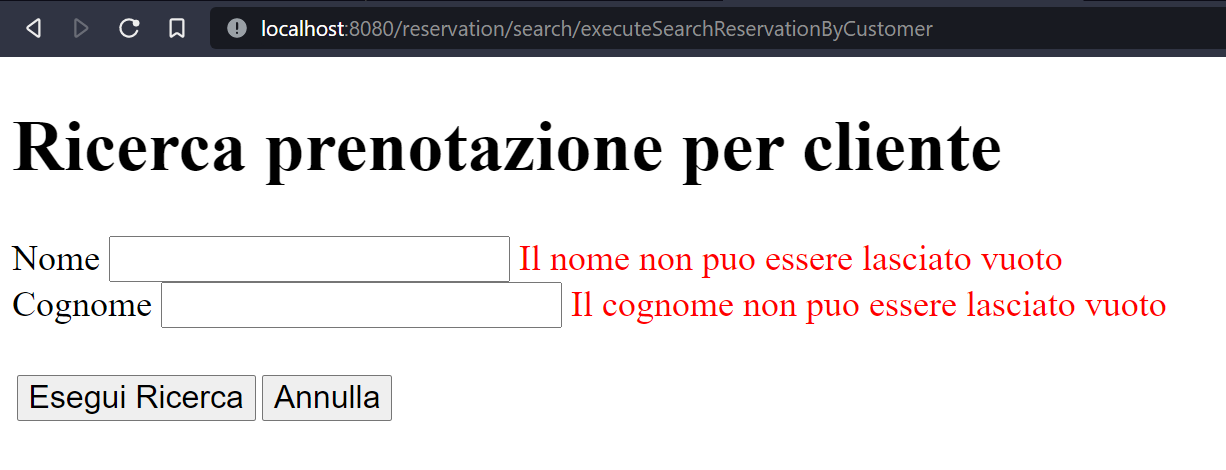
\includegraphics[width=0.9\textwidth]{images/search_reservation_by_customer_errors}
        \label{fig:search_reservation_by_customer_errors}
        \caption{Searching a reservation by customer violating requisites}
    \end{figure}

    \vspace*{5mm}

    \subsection*{Search Reservation by Date}
    \label{sec:search_reservation_by_date_errors}
    \begin{figure}[H]
        \centering
        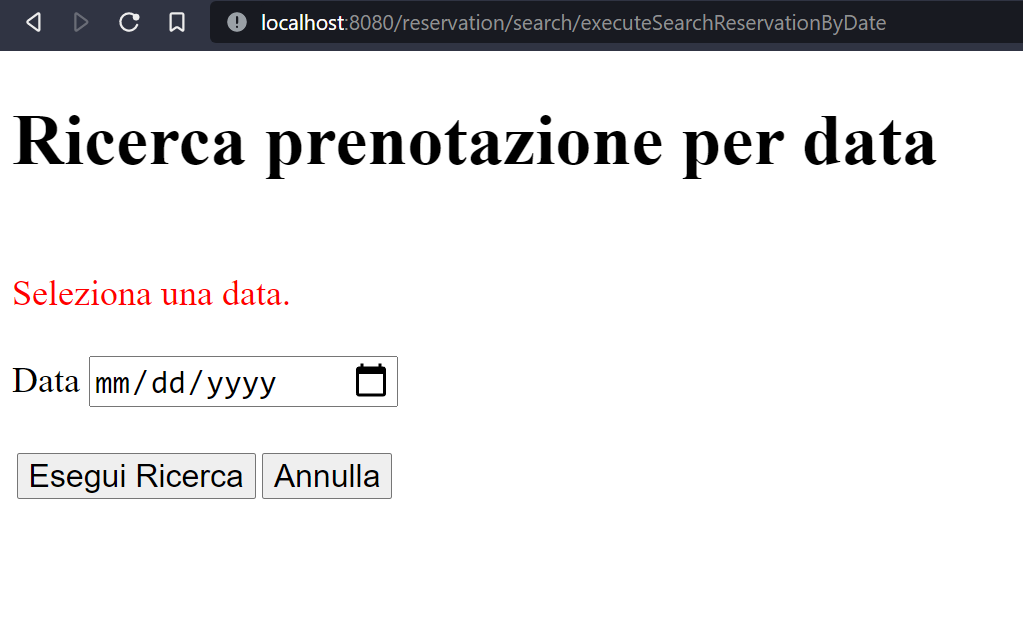
\includegraphics[width=0.9\textwidth]{images/search_reservation_by_date_errors}
        \label{fig:search_reservation_by_date_errors}
        \caption{Searching a reservation by date violating requisites}
    \end{figure}

\end{document}
